%!TEX root = ../thesis.tex
%*******************************************************************************
%*********************************** First Chapter *****************************
%*******************************************************************************

\chapter{Introduction}\label{chap:intro}  %Title of the First Chapter

\ifpdf
    \graphicspath{{Chapter1/Figs/Raster/}{Chapter1/Figs/PDF/}{Chapter1/Figs/}}
\else
    \graphicspath{{Chapter1/Figs/Vector/}{Chapter1/Figs/}}
\fi


%********************************** %First Section  **************************************
\section{Motivation} %Section - 1.1 

Animal welfare is an important concern for business and society, with an estimated 70 billion animals currently living under human care~\cite{FAOSTAT}. Across multiple industries, monitoring and assessing animal health is achieved by measuring individuals' body shape and movement. These measurements should be taken without interfering with the animal's normal activity, and are needed around the clock, under a variety of lighting and weather conditions, perhaps at long range (e.g.\ in farm fields or wildlife parks). 

Of course, employing humans to monitor large animal populations is costly and can lead to data bias. For example, prey animals such as rodents are known to alter their behaviour in the presence of perceived predators. To overcome this, there is a developing field of literature which focuses on automatic animal monitoring. Many of of these are specifically designed for use in pre-clinical work. Some systems measure animals ``invasively'', meaning they surgically implant a measuring device. Although these systems can offer detailed biometric data (such as blood pressure, ECG etc.), a stressful implantation procedure is often required which can lead to complex behavioural effects which are difficult to model.

This motivates the design of \emph{non-invasive} systems which rely on other means, including cameras, to monitor animal populations. Even simple examples of these can be surprisingly effective. For example, a reliable pixel-based motion detector can be used to indicate the most basic of health standards -- that the animal is at least alive. More advanced systems are able to estimate animal behaviour, energy and inquisitiveness levels of target animals by analysing activity patterns over time. Basic analysis can be achieved by mechanical means, such as by installing floor-level pressure pads~\cite{zammit2010reliability}, but deeper insights are generally afforded through computer vision algorithms processing images obtained from camera systems.

Techniques that represent animal behaviour using cameras for health and welfare analysis can be grouped into two categories. The former class treat animal behaviour as a machine learning classification task, in which a computer is taught to visually recognize predefined activities using a large collection of manually annotated videos. For `normal' behaviours (e.g. drinking, eating etc.) this is a viable approach and health insights can be inferred by monitoring the pattern of these over time. However, systems of this kind cannot readily be extended to identify more serious conditions (e.g. animals experiencing a seizure), due to the ethical concerns associated with collecting examples of adverse behaviours for system training. 

To overcome this concern, and reduce annotation effort, the second class of approaches take inspiration from `proxy' representations of human beings, which have been recently popularized in computer vision literature. Following work in human pose estimation, some methods design discriminative body part recognizers or keypoint predictors in order to represent animal subjects as a sparse set of control point (often termed \emph{joints}) locations. This representation offers a number of advantages. Firstly, data collection for this proxy representation is quicker and cheaper since it can be completed by non-expert annotators. Secondly, the representation preserves most important details so can be used in a pipeline with a downstream algorithm to produce the desired output. For example, one may directly measure the joint trajectories to estimate the animal's balance. Thirdly, downstream machine learning algorithms typically require much less task-specific training data since nuisance factors (e.g. background, textures etc.) have already been removed. Finally, for data retention purposes, recording per-frame keypoints is much less cumbersome and more easily searchable than raw pixel data.

However, it is natural to question whether abstracting animals as a set of keypoints is sufficient to facilitate all downstream applications. Unfortunately, the answer to this is `no'. While a sparse keypoint representation is generally enough to capture the animal's \emph{pose} (e.g. limb positions), nearly all body \emph{shape} information is lost. This prevents diagnostics which are often mandatory in pre-clinical settings. For example, keypoints alone cannot be used to measure an animal's weight or breathing rate. Therefore, this thesis contributes to a class of approaches which recover the 3D structure of an animal, including \emph{both pose and shape} information from an input image or video sequence.

% In most clinical applications, these metrics are often mandatory and, importantly cannot be estimated from keypoints alone. 


% Tthe animal's skeleton can be recovered   However, this thesis argues that despite the benefits, such a representation is too limited for health monitoring purposes. For example, such a representation 

% by installing an overhead camera and designing computer vision algorithms. Examples include systems which performs simple visual blob detection via colour thresholding~\cite{tort2006simple}, \cite{rodriquez2017toxtrac}. Which such systems are effective at tracking animals with distinctive colour using fixed cameras in areas with consistent backgrounds, these systems do not generalize well to more challenging scenarios, particularly outdoors. The presence of changing light levels, casting of shadows across tracking targets or moving backgrounds (e.g.\ foliage) make setting appropriate thresholds difficult and other factors, such as occlusion caused by the environment or other animals/humans are difficult to resolve.

% Some work has been done in automatic behavioural scoring for rodents, in which up to ten predefined behaviours can be visually recognized. These approaches typically employ machine learning algorithms, which are taught to recognize behaviours present in a video stream by analyzing a large set of pre-collected examples. For `normal' behaviours (e.g. drinking, eating etc.) this can be a viable approach and by analyzing the changing frequency of such behaviours can indeed offer insights into underlying conditions. However, these systems cannot be readily extended to handle more serious conditions (e.g. animals experiencing a seizure), due to the ethical concerns associated with collecting examples of such behaviours for system training. 

% This thesis proposes an alternative strategy 

% In addition, many 
% Of course, even if a behaviour detection system were built for a range of animal species this 

% % TODO: Explain why these are of limited use for robust 3D tracking.
% % -> Cannot collect behavioural training data for adverse effects
% % -> Weight estimation
% % -> Platform for future machine learning tools

% % Say that we want it to be cheap!

% Unfortunately, all these approaches suffer as they fail to reconstruct a full 3D mesh.

% Between farmyards, research facilities, zoos, animal rescue centres, veterinary centres and sporting centres, over 100 billion animals are currently living under human care \cite{FAOSTAT}. For ethical and financial reasons, these industries often rely on the health and wellbeing of their animal populations and there can be dramatic consequences afforded to organizations deemed to fall short. Pressure groups have been particularly critical of zoos and entertainment industries for their inability to identify and treat behaviour disorders. In some cases, this has necessitated expensive re-homing procedures for animals with late-identified psychosis (commonly stereotypy)~\cite{Guardian-Elephant}. Worse still, some have suggested a link between animal health and welfare and loss of human life~\cite{SWOH-Tilikum}.

% This project is funded by GlaxoSmithKline (GSK), a global pharmaceutical company based in the United Kingdom. In order to sell medications for use in humans, GSK and similar companies have a legal obligation to run controlled clinical trials on animal subjects. For reasons of ethics and promotion of good science, the emphasis on animal welfare is paramount. Strict measures are imposed to minimize any potential animal suffering and to maximize useful data output during the study period. By refining existing methods of behaviour analysis, GSK aim to further reduce the numbers of animals required for testing and support robust conclusions about candidate medications at earlier opportunities. Progress here should assist scientists in identifying medicinal side-effects and promote early attrition of the clinical trial, that is, the process of preventing an unsuitable drug compound from progressing in the R\&D pipeline and thereby reducing any further unnecessary expenditure.

% Within sectors concerned with animal husbandry, there is growing support for a system able to continuously monitor captive animals throughout their entire lifetimes. Due to staff working hours and typically large population sizes, it can be impractical for zookeepers or lab technicians to keep continuous watch over all animals under their care at all times. These issues are particularly acute for nocturnal animals in which symptoms may only become apparent during the night, and `prey' animals that have evolved to deliberately hide pain from perceived predators as a defence mechanism. Rats and mice, the two most common species used in animal research, pose both of these challenges.

%********************************** %Second Section  *************************************
\section{Approach} %Section - 1.2

% This thesis focuses on developing methods for recovering a 3D model of an animal oa tracking system to enable recovery of a per-frame 3D animal reconstruction from an image or video stream. 

% The system should apply to a wide range of animal species without significant customization. Success in this endeavour would enable real-time changes of a known skeletal structure to be programmatically analysed to completely model an animal’s movements. These behaviour patterns could then be interpreted to form a profile for each animal in a batch, taking into account expected norms for their species as well as their individual personality traits. When animals are first brought into a facility, they are given some time to acclimatize to their new surroundings before a clinical study begins. The application could make use of this period to refine behaviour models to their particular characteristics without being influenced by external factors. The system would then begin monitoring the population, storing detailed analytics and reacting to any deviations to an animal’s unique behaviour profile. As a simple example, should a typically lively and sociable dog suddenly begin exhibiting signs of withdrawal from the group, this would indicate a cause for concern and be stored in that animal’s ‘virtual log book’. In some cases, an animal may begin to exhibit signals that demand immediate attention, such as a dramatic and sudden energy drop that may indicate pain. The application could handle such events by sending an SMS text message to an on-call veterinary professional, to alert them of the specific problem and thereby enable a rapid response. These real-time diagnostics could then be aggregated and displayed on a dashboard screen, visible to all laboratory technicians. A concept drawing is shown in Figure \ref{fig:wellness_dashboard}.

% \subsection{Problem definition}
This thesis tackles the problem of recovering dense 3D reconstructions of animals from monocular images or video. Of course, humans generally have no problem with this task. In particularly, humans are generally capable of predicting, at least approximately, the 3D structure of most scenes including animal subjects, even from a single viewpoint. However, the visual evidence present in a single 2D image notoriously~\citep{Faugeras01geometry} contains insufficient information for the third dimension to be recovered unambiguously. Having access to a full video sequence does help somewhat, although significant sources of ambiguity remain due to camera motion, animal limb movement and occlusion caused by environment or other objects. 
To assist, this thesis follows a common strategy, popularized in 3D human mesh reconstruction literature, which incorporates strong prior knowledge over the target subject class to reduce the reconstruction ambiguity. This prior can be factored into two components: a \emph{shape} prior that enforces topological (e.g.\ order of body parts) and measurement constraints (e.g.\ length of limbs), and a \emph{pose} prior that defines likely limb configurations and can be used to rule out those which are anatomically impossible. 
In this thesis, the prior takes the form of a \emph{3D morphable model} -- a parameterized 3D mesh model which can be adapted to match the input animal.

\begin{figure}[t]
    \centering
    \begin{subfigure}{0.33\textwidth}
    \centering
        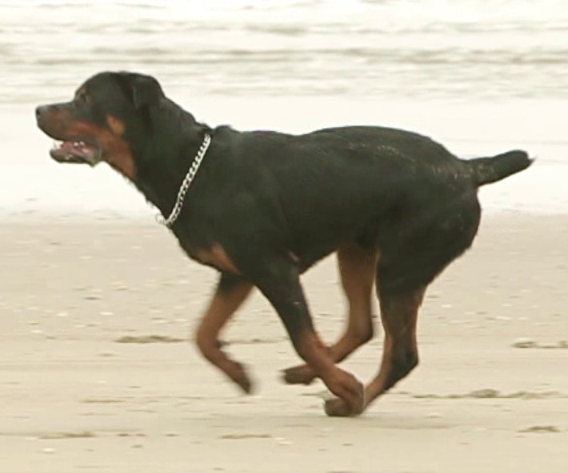
\includegraphics[width=1\linewidth]{input/66}
    \end{subfigure}%
    \begin{subfigure}{0.33\textwidth}
    \centering
        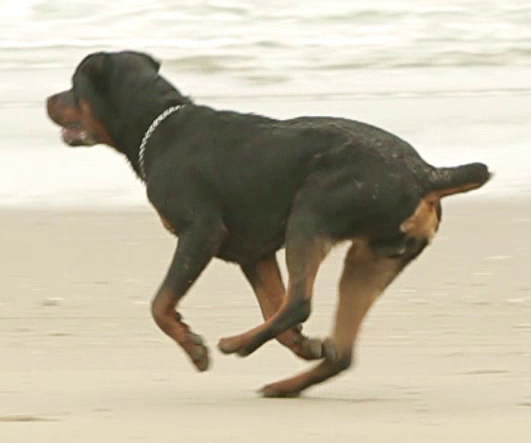
\includegraphics[width=1\linewidth]{input/167}
    \end{subfigure}%
    \begin{subfigure}{0.33\textwidth}
    \centering
        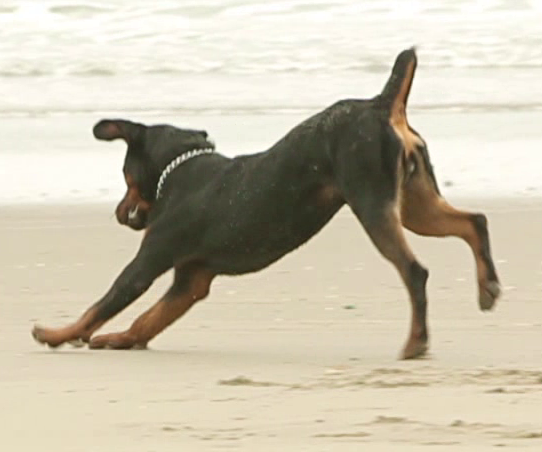
\includegraphics[width=1\linewidth]{input/208}
    \end{subfigure}%
    \caption{An example input video sequence.}
    \label{fig:arap_input}
\end{figure}

    % An example output showing the recovery of a 3D model from an input 2D monocular video is shown in Figure \ref{fig:intro_arap_output}:
    
    % \begin{figure}[H]
    %     \centering
    %     \begin{subfigure}{1\textwidth}
    %     \centering
    %         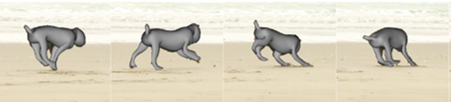
\includegraphics[width=1\linewidth]{input/arapsfm_output}
    %     \end{subfigure}%
    %     \caption{Sample output printed from Deformable Mesh Animation~\cite{arap_stebbing}.}
    %     \label{fig:intro_arap_output}
    % \end{figure}

As alluded to in the previous section, a distinction should be made between two common tracking techniques: (1) discriminative body part recognizers and joint position predictors, and (2) 3D reconstructions via generative model fitting. Discriminative predictors are a popular alternative to full mesh recovery, and have facilitated common use-cases, such as gesture detection or controllerless gameplay. However, to enable animal \emph{shape} recovery, the work in this thesis is closer to approaches that recover full 3D surface models of human subjects. Applications are found in fashion to facilitate online `try-ons' for virtual clothing~\cite{lin2014digital}, in animation and visual effects to generate virtual characters from live actor performances~\cite{laine2017production}, and in healthcare for tracking patients' body weight over time~\cite{velardo2010weight}. 

%It is hypothesized that recovering a full 3D animal reconstruction is necessary to enable the intended diagnostic purposes of this animal work. In particular, returning only joint positions or body parts may be insufficient to estimate animal weight. If this can be realized, identifying behavioural changes from the reconstruction is expected to be a relatively straightforward machine learning problem. 

A typical method for recovering 3D structure from articulated subjects is via a \emph{model fitting} approach, in which a representative 3D morphable model is adapted to recreate the performance of the target. This method involves: (1) designing a suitable 3D morphable model with shape and pose parameterized that represent the target animal species, and (2) designing a machine learning algorithm which operates on an input image or video sequence and outputs per-frame parameters. An example of a template mesh is shown in Figure~\ref{fig:arap_template}.

\begin{figure}[t] % Example image
    \center{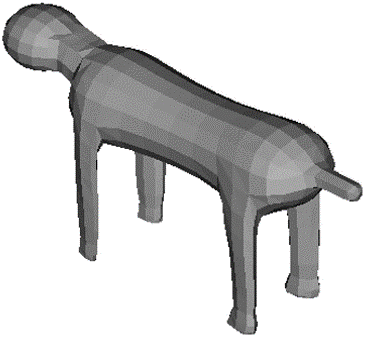
\includegraphics[width=0.2\linewidth]{template_mesh}}
    \caption{An example prior, in this case a template mesh.}
    \label{fig:arap_template}
\end{figure}

Shape attributes capture variation between different members of the target class and therefore remain fixed for a particular individual. For example, shape parameters may be adapted to vary a model's height and weight. However, pose attributes capture limb positions and joint angles, and therefore tend to vary considerably between frames of a capture sequence. Figure~\ref{fig:black_shape} highlights the difference by keeping pose parameters fixed while shape attributes are varied between the three models~\cite{Streuber:SIGGRAPH:2016}.

\begin{figure}[t] % Example image
    \center{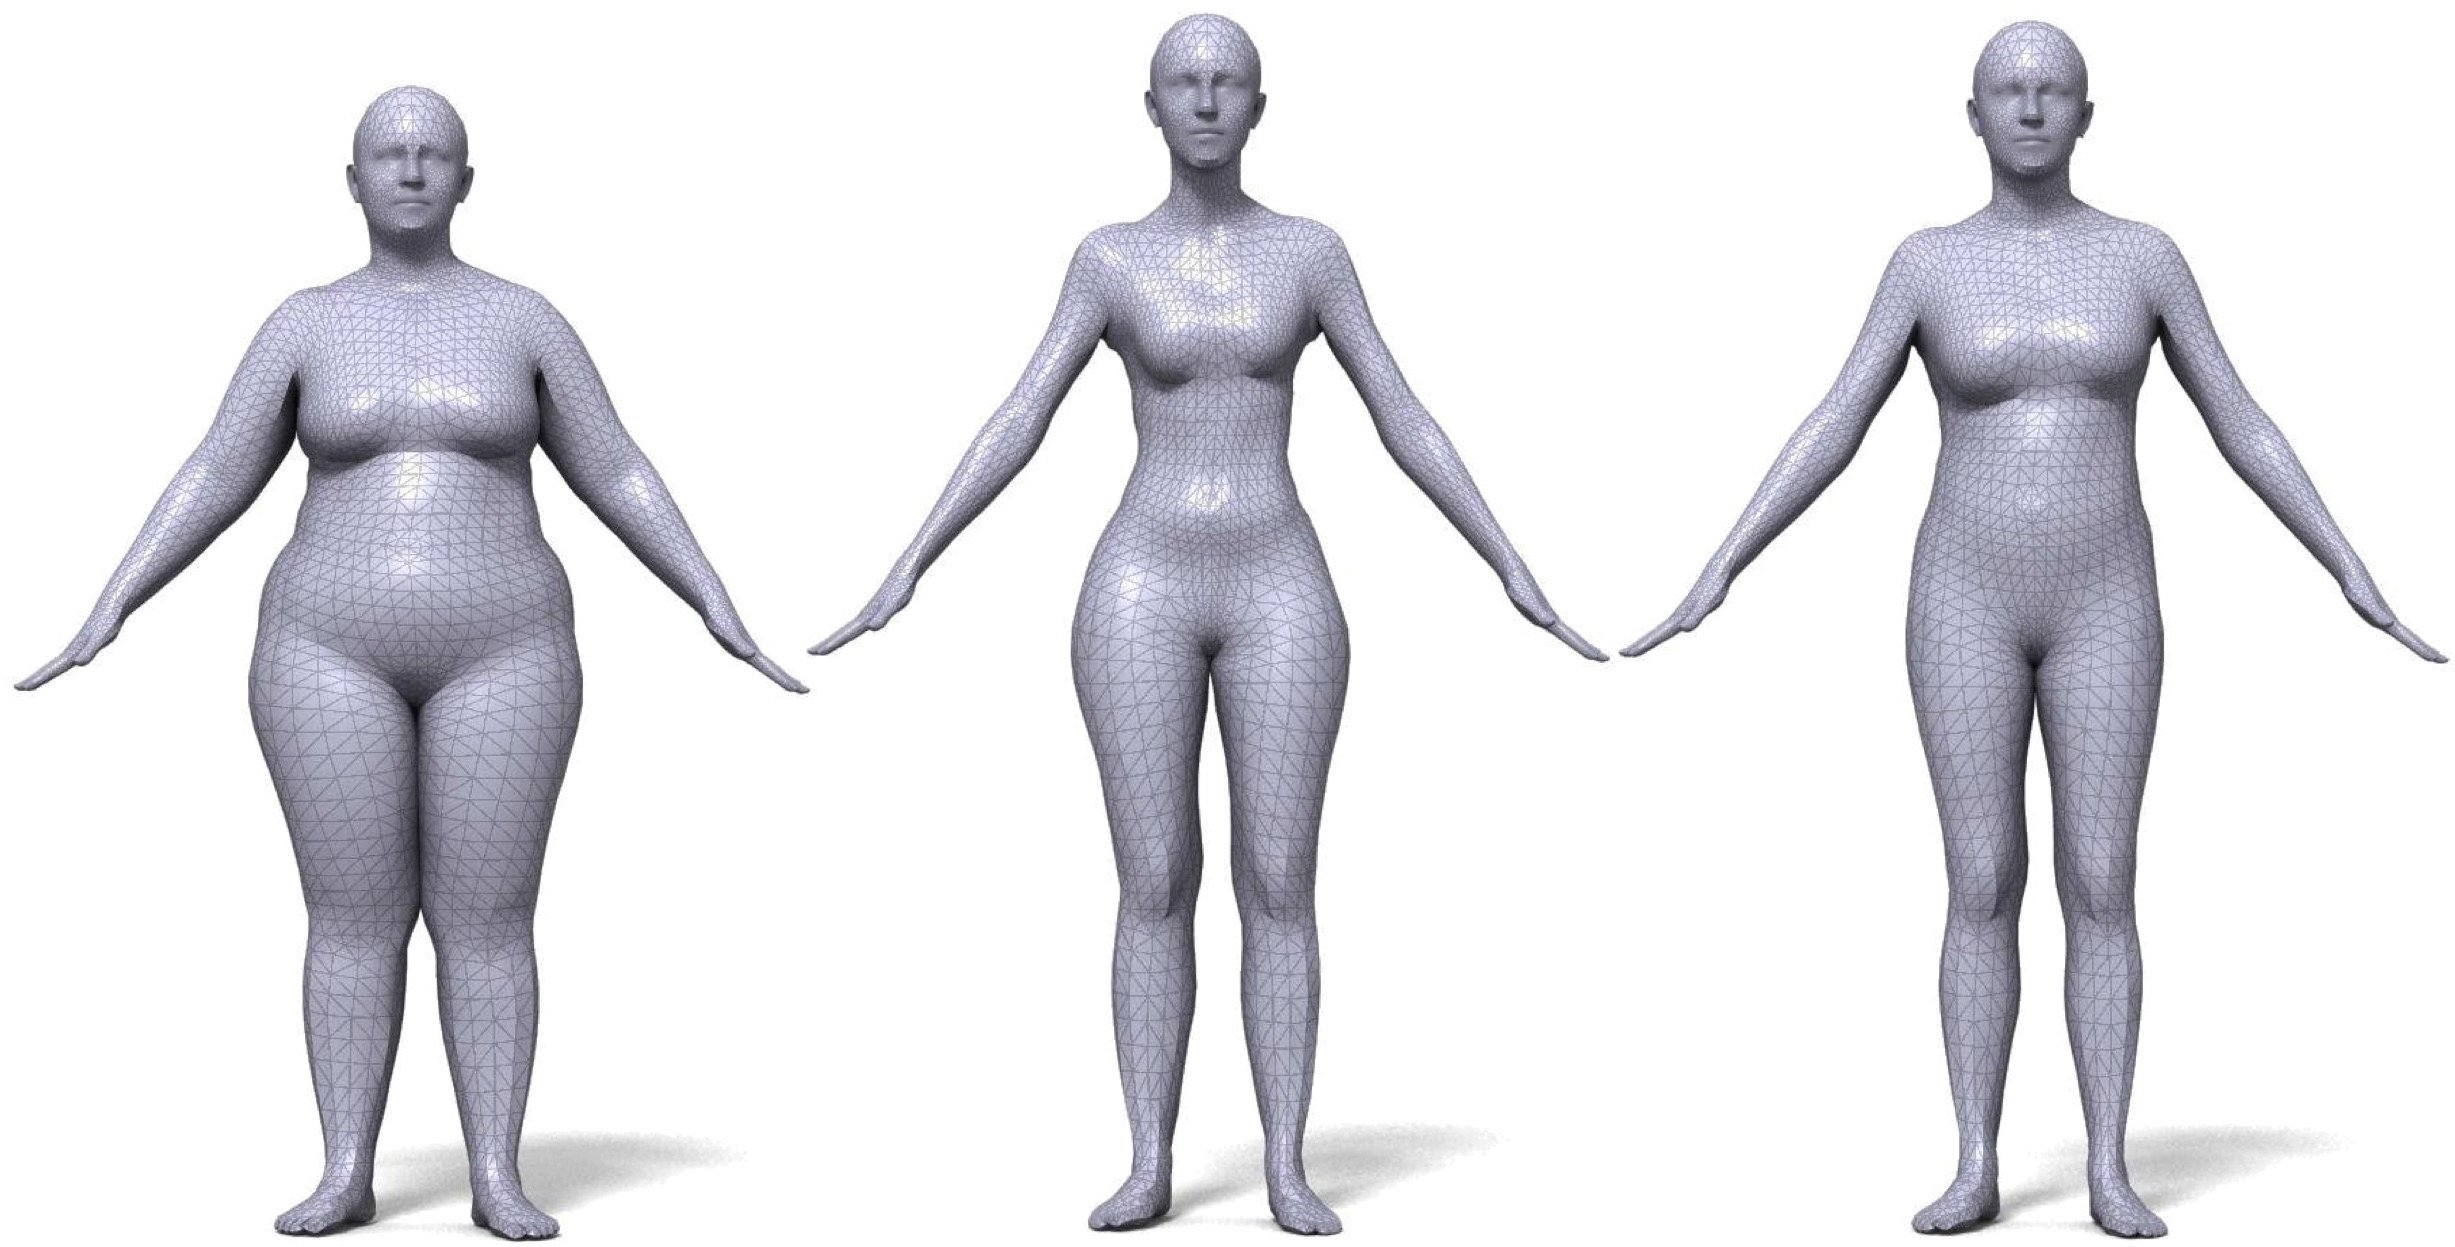
\includegraphics[width=0.9\linewidth]{body_shapes}}
    \caption{Varying human shape parameters while pose remains fixed. Reprinted from~\cite{Streuber:SIGGRAPH:2016}.}
    \label{fig:black_shape}
\end{figure}

Once shape and pose parameters have been derived from a video sequence, they can be applied to the template mesh to generate a digital version of the same activity. If successful, the changing parameters should appear to adapt the template mesh such that it faithfully reproduces the activity of the original animal. 

%In early experimentation, in which tracking targets are restricted to the same species, the template can be chosen to be a close shape fit to the target animal, thereby largely reducing the problem to finding optimal per-frame pose parameters. However, tracking examples are eventually broadened to include a wide range of animal species.

\section{Relation to human reconstruction}
% NEEDS TIDYING
In recent times, 3D human reconstruction has become an established computer vision subfield. It is therefore natural to question to what extent techniques developed for this purpose transfer to the animal case. Some aspects of this are considered:

% Of course, there is some overlap in challenges between animal and human subjects, most notably in the need to reconstruct self-deforming objects which frequently self-occlude. However, additional challenges are posed for animals due to the complex diversity in shape, pose and texture between animal tracking candidates, the limited availability of 3D data for training algorithms and the prevalence of environmental/object occlusion, particularly in internet animal imagery.  However, one advantageous aspect when tracking animals over humans is the simple fact that animals tend not to wear clothing, which in humans causes significant shape and appearance variability.


\subsection{Self-deforming objects.} Animal and human subjects can control their limb positions for the purposes of movement and expression. Modelling the space of allowable motion is generally important to ensure reconstructions are anatomically plausible. For quadrupedal animals, limb reasoning can be made more difficult due to four legs (rather than two for humans) in rapid motion in a small area. This increases self-occlusion and can make it more challenging to distinguish between pairs (e.g.\ left/right and back/front).

\subsection{Variability.}
The variation of shape across and within animal species is considerably greater than in humans and variations in surface texture are considerably larger and more complex than in humans. One advantageous aspect of tracking animals rather than humans is that animals generally do not wear clothing. 

% In one sense, AT is simpler than human tracking as animals generally do not wear clothing. However, variations in surface texture are still considerable between individuals, and the variety of shape across and within species is considerably greater.  If tracking is specialized to a particular species, then shape variation is smaller, but training data is even harder to obtain.

\subsection{Training data.}
For human tracking, hand labelled sequences of 2D silhouette segmentations and joint positions have been collected from a wide variety of sources~\cite{andriluka14cvpr,lin2014microsoft,johnson2010clustered}. Of these two classes of labelling, animal {\em segmentation} data is available in datasets such as MSCOCO~\cite{lin2014microsoft}, PASCAL VOC~\cite{everingham2010pascal} and DAVIS~\cite{Perazzi2016}.  However this data is considerably sparser than human data, and must be ``shared'' across species, meaning the number of examples for a given animal shape class is considerably fewer than is available for an equivalent variation in human shape.  While segmentation data can be supplied by non-specialist human labellers, it is more difficult to obtain {\em joint position} data.  Some joints are easy to label, such as ``tip of snout'', but others such as the analogue of ``right elbow'' require training of the operator to correctly identify across species.

Of more concern however, is 3D skeleton data.  For humans, motion capture (mocap) can be used to obtain long sequences of skeleton parameters (joint positions and angles) from a wide variety of motions and activities.
For animal tracking, this is considerably harder: animals behave differently on treadmills than in their quotidian environments, and although some animals such as horses and dogs have been coaxed into motion capture studios~\cite{wilhelm2015furyexplorer}, it remains impractical to consider mocap for a family of tigers at play.

% The previous chapter discussed the primary objective of this work, which is to recover full 3D shape and pose from a live input video sequence exhibiting an animal subject. As explained, the major challenge common to all methods operating on monocular RGB input is to resolve the inherent depth ambiguity associated with recovering a 3D model from 2D input. Competitive methods achieve this by relying on strong motion cues~\cite{kinect_fusion} or (if available) by incorporating strong prior knowledge of the tracking target. Strong shape and pose priors (e.g. body part configuration, acceptable body part lengths, likely joint positions etc.) are available for this problem, so this report will focus on analysing these methods in the literature.

% All solutions face an important design decision, which is to make a distinction between features of an input sequence the system should aim to model and to which it should remain invariant. For example, nearly all human systems aim to model the angle between a tracking target's upper and lower leg region, but nearly all will attempt to remain invariant to skin colour variation between candidates. The next two sections discuss examples of systems in which this decision has been made differently, generally according to the intended real-world application.

% We address this problem using techniques from the recent human body and hand tracking literature, combining machine learning and 3D model fitting.  A discriminative front-end uses a deep hourglass network to identify candidate 2D joint positions. These joint positions are then linked into coherent skeletons by solving an optimal joint assignment problem, and the resulting skeletons create an initial estimate for a generative model-fitting back-end to yield detailed shape and pose for each frame of the video.  

% Although superficially similar to human tracking, animal tracking (AT) has some interesting differences that make it worthy of study:

% \subsubsection*{Variability.}
% In one sense, AT is simpler than human tracking as animals generally do not wear clothing. However, variations in surface texture are still considerable between individuals, and the variety of shape across and within species is considerably greater.  If tracking is specialized to a particular species, then shape variation is smaller, but training data is even harder to obtain.

% \subsubsection*{Training data.}


% \begin{figure}[H] % Example image
%     \center{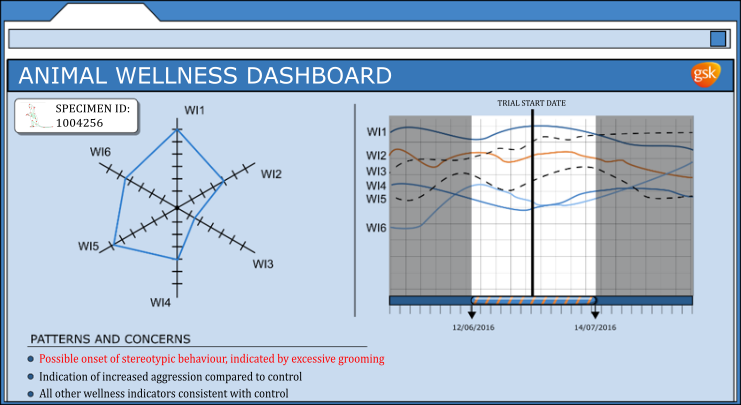
\includegraphics[width=0.95\linewidth]{dash}}
%     \caption{Concept drawing showing an animal health dashboard. Specific wellness markers WI1,...,WI6 have yet to be determined.}
%     \label{fig:wellness_dashboard}
% \end{figure}


%********************************** % Third Section  *************************************
\section{Contributions}  %Section - 1.3 
This thesis tackles key challenges associated with deriving 3D dense reconstructions of animal subjects from monocular input images and video sequences. \Cref{chap:relwork} contains an in-depth literature review of works focusing on 3D reconstruction of articulated subjects. Specific attention is put towards approaches for designing 3D morphable models, and strategies for predicting the parameters from input data. 

\Cref{chap:cgas} introduces an approach for 3D animal reconstruction and overcomes the limited availability of real world 3D training data for animals by generating synthetic training images. A deep neural network is trained on these images and tested on real world examples to produce joint heatmaps. Importantly, generalization to real test set sequences is ensured by extracting silhouettes. Optimal joint locations are extracted from predicted heatmaps using a discrete optimization, before a model fitting procedure recovers the full 3D animal model. The method is tested on a range of animal videos and is the first to demonstrate full 3D animal mesh recovery with with no required user intervention. 

\Cref{chap:wldo} describes an end-to-end and real-time neural network which recovers accurate 3D reconstructions for the challenging dog category, trained using weak 2D supervision. The chapter introduces SMBLD, a new 3D deformable template model which includes additional limb scaling parameters and a detailed shape prior learnt according to an Expectation Maximization procedure during network training. The method is shown to be state-of-the-art on a new StanfordExtra dataset, the largest of its kind for animals, improving over competitive energy minimization techniques even when they are given access to ground truth data. 

\Cref{chap:3dmulti} tackles the problem of recovering 3D reconstructions when given input images exhibiting significant sources of ambiguity, such as environmental occlusion or a partial views of the subject. Rather than attempting to recover a reconstruction uniquely, a multi-hypothesis neural network outputs a set of plausible and varied reconstructions which are all consistent with the input image. The network is trained according to a best-of-$M$ loss, to which flexibility is added using a novel quantization scheme based on normalizing flows. 

\section{Co-Authored Papers}  %Section - 1.4

This thesis is derived in part from three co-authored publications. \Cref{chap:cgas} contains work from:

\begin{quote}
    \textbf{Benjamin Biggs}, Thomas Roddick, Andrew Fitzgibbon and Roberto Cipolla. \emph{Creatures Great and SMAL: Recovering the Shape and Motion of Animals from Video}. ACCV 2018, Oral Presentation.
\end{quote}

\noindent
\Cref{chap:wldo} contains work from:

\begin{quote}
    \textbf{Benjamin Biggs}, Oliver Boyne, James Charles, Andrew Fitzgibbon and Roberto Cipolla. \emph{Who Left the Dogs Out? 3D Animal Reconstruction with Expectation Maximization In the Loop}. ECCV 2020.
\end{quote}

\noindent
\Cref{chap:3dmulti} contains work from:

\begin{quote}
    \textbf{Benjamin Biggs}, Sebastien Ehrhadt, Hanbyul Joo, Benjamin Graham, Andrea Vedaldi and David Novotny. \emph{3D Multi-bodies: Fitting Sets of Plausible 3D Human Models to Ambiguous Image Data}. NeurIPS 2020, Spotlight Presentation.
\end{quote}